
\documentclass[10pt,letterpaper]{article}
\usepackage[top=0.85in,left=0.85in,footskip=0.75in]{geometry}
% amsmath and amssymb packages, useful for mathematical formulas and symbols
\usepackage{amsmath,amssymb}
% Use adjustwidth environment to exceed column width (see example table in text)
\usepackage{changepage}
% Use Unicode characters when possible
\usepackage[utf8x]{inputenc}
% textcomp package and marvosym package for additional characters
\usepackage{textcomp,marvosym}
% cite package, to clean up citations in the main text. Do not remove.
\usepackage{cite}
\usepackage{url}
% Use nameref to cite supporting information files (see Supporting Information section for more info)
%\usepackage{nameref,hyperref}
% line numbers
%\usepackage[right]{lineno}

%\usepackage{natbib}
\usepackage{graphicx}
\usepackage{float}

% color can be used to apply background shading to table cells only
\usepackage[table]{xcolor}

% array package and thick rules for tables
\usepackage{array}
\usepackage{dsfont}

\usepackage{todonotes}
\usepackage{comment}

% referencing supplement-material
\usepackage{xr}
\externaldocument{./supplement}
%\usepackage{cleveref}



%% END MACROS SECTION

\title{Triqler for Protein Summarization of Data from Data Independent Aquisition Mass Spectrometry}
\author{Patrick Truong \and Matthew The \and Lukas K\"{a}ll}


\begin{document}
%\linenumbers
\maketitle

%Here I want to reference a figure that is in my supplementary content \cref{supp-fig:model_selection_criteria}.

%Here is a ref to the supplement, we have a Supplementary Figure \ref{fig:diff_vs_hela_find_a_better_label}.

\begin{abstract}

Within mass spectrometry-based proteomics, protein summarization and quantification is recognized as complex problems. The detection and quantification of each proteoform's protolytic peptides is an error-prone process, and there is a need for computational methods to assess errors and determine which measurments that can be trusted or not.  We have previously designed a integrative model, Triqler, that combines identification and quantification errors and summarize results into protein quantities. 
Here we show that Triqler, is well compatible with data-independent acquisition data, despite being designed for data-dependent acquisition data. Furthermore, we find that it has better performance than other protein summarization tools, when evaluating a relatively large set of different DIA processing methods. 

\end{abstract}
  

\section*{Introduction}

Label-free quantification (LFQ) using Mass spectrometry (MS)-based proteomics enables efficent determination of differential concentrations of proteins in complex mixtures. The processing of data from such experiments requires multiple different steps, all subjects to errors. 
For the analysis of mass spectrometry-based proteomics data, just as any other type of analysis of complex data, the individual computational methods for all the steps in the processing affect the final results. It is therefore quite hard to evaluate the influence of the individual tools, which should not stop the field from trying to establish what the features of the different processing steps \cite{dufresne2014abrf,gatto2016testing,navarro2016multicenter}. Unbiased comparisons of software tools is challenging for several reasons \cite{dufresne2014abrf}. Methods can be assessed by scientist lacking relevant expertise, the tested methods may be lacking sufficient documentation and the interpretation of test results may be subjective \cite{yates2012toward} \cite{leprevost2014best} \cite{pak2013clustering} \cite{faircomparison2015}. By using the same data set we can assure that the data set is processed consistently and further the analysis by extending it to protein summarization procedures.


We have previously designed a hierarchical Bayesian model, Triqler, able to control for errors from both the identification and quantification process in such experiments\cite{The2018Integrated}. By integrating the errors probabilities from identification and quantification one can obtain better accuracy in calling differentially abundant proteins \cite{The2018Integrated}.   Triqler was designed for handling LFQ data from Data-dependent acquisition (DDA). However, many labs prefer Data-independent acquisition (DIA) mass spectrometry \cite{venable2004automated} as they find that it gives more reproducible peptide detection, and allow for a broader dynamical range in quantification \cite{bern2010deconvolution,zhang2020DIA}, compared to DDA. 

Here, we set out to investigate Triqler ability to summarize protein concentrations from peptide abundances deduced from DIA data. We primarly used the LFQBench from Navarro et al. \cite{navarro2016multicenter} for the evaluation. In the original benchmark, Navarro et al. included a comaprison of different protein summarization strategies, and found that the so-called Top3 method generally resulted in lower variance and better quantification accuracy than the built-in methods from the tested methods\cite{navarro2016multicenter}. However, there are reasons to believe that more sophisticated methods would yield better protein quantification than the Top3-method. Simple summarization methods based on mean and median peptide intensity has been shown to produce unreliable protein abundance estimates \cite{goeminne2015summarization}, and more advanced summarization strategies for LFQ data has been proposed in literature \cite{silva2006absolute,cox2014accurate}, and summarization techniques such as PQPQ~\cite{forshed2011enhanced}, msStats~\cite{choi2014msstats}, Diffacto~\cite{zhang2017covariation}, MSqRobSum~\cite{sticker2020robust} and Triqler~\cite{The2018Integrated} has all been shown to outperform Top3 and there currently exists no reason why said methods would not theoretically be able to perform well for DIA data. Hence, we found it apt to benchmark Triqler against a set of state-of-the-art protein summarization methods using peptide quantities from the LFQBench DIA data set.


% Here, we found a previous data set most useful for the comparison of methods, the LFQBench from Navarro et al. \cite{navarro2016multicenter} constructed a high-quality data set for five widely used tools for analysis of SWATH-MS data (four peptide-centric query tools: OpenSWATH \cite{rost2014openswath}, SWATH 2.0, Skyline \cite{maclean2010skyline}, Spectronaut \cite{bruderer2015extending}, and one data-centric approach DIA-Umpire \cite{maclean2010skyline}), which is readily amendable for a benchmark of other methods.
 
 
\section*{Materials and methods}


\subsection*{Data description}
\subsubsection*{Mass spectrometry data}


We downloaded the LFQBench dataset~\cite{navarro2016multicenter} from PRIDE identifier PXD002952. Here we used the TripleTOF6600 (ABSciex) section of the study, which was harvested with a setup of 32 fixed windows ms2-windows. We also restricted ourselves to the low ratio difference samples, reffered to as the HYE124 hybrid proteome samples in the original study. That consists of triplicates of Sample A composed of tryptically digested proteins from 65\% w/w HeLa, 30\% w/w yeast, and 5\% w/w \textit{E. coli} cells, and triplicates of Sample B, composed of 65\% w/w, 15\% w/w yeast, and 20\% w/w \textit{E. coli} proteins. Samples from HYE110 and the TripleTOF5600 section of HYE124 was omitted in this study. Further details about mass spectrometric instrumentation and data acquisition are available in Navarro et al.~\cite{navarro2016multicenter}. The \verb|.wiff| files were converted to \verb|.mzML| files in a centroided format using msconvert (using windows OS msconvert version 3.0) with peakPicking filter msLevel=1-). 


\subsubsection*{Sequence database}

Uniprot FASTA files with one protein sequence per gene was downloaded for each species (UP000005640, UP000000625, and UP000002311, acquired on 2021-06-16). The unfiltered FASTA files contained 20 590 human proteins, 6 046 yeast proteins, and 4 373 \textit{E. coli} proteins. To reduce for the effect of the different protein inference strategies for the tested protein summarization tools, a modified .fasta file, without shared peptides, was used for database search. The filter randomly removed protein sequences with shared peptides, so that the final database did not contain any tryptic peptides with length $>$7 amino acids mapping to peptides shared with other proteins. After filtering the FASTA file contained 20 302 proteins (288 human proteins less proteins than unfiltered database), 5 848 yeast proteins (198 yeast proteins less proteins than unfiltered database), and 4 306 \textit{E. Coli} proteins (67 \textit{E. Coli} proteins than unfiltered database). Replacing the I/L amino acids with to handle mass-equivalence did not result in any considerable differences (See Supplementary Table \ref{table:proteins_in_database}). We also added pseudo-reverse sequences to the database as decoys for target-decoy analysis using OpenSwathDecoyGenerator. 

\subsection*{General workflow}

Just as in LFQBench, we used two separate strategies to generate peptide abundances from the DIA-runs, first we used a spectral library consisting of selected spectra from separate DDA runs, we refer to this workflow as DID hereon, and second we searched pseudo-spectra generated directly from the DIA data, we will refer to this workflow as PS from hereon. The workflows are shown in figure \ref{fig:flowchart}. We will describe the parameter choices of both theses two methods below.

\begin{figure}[htp]
    \centering
    \begin{tabular}{lclc} 


        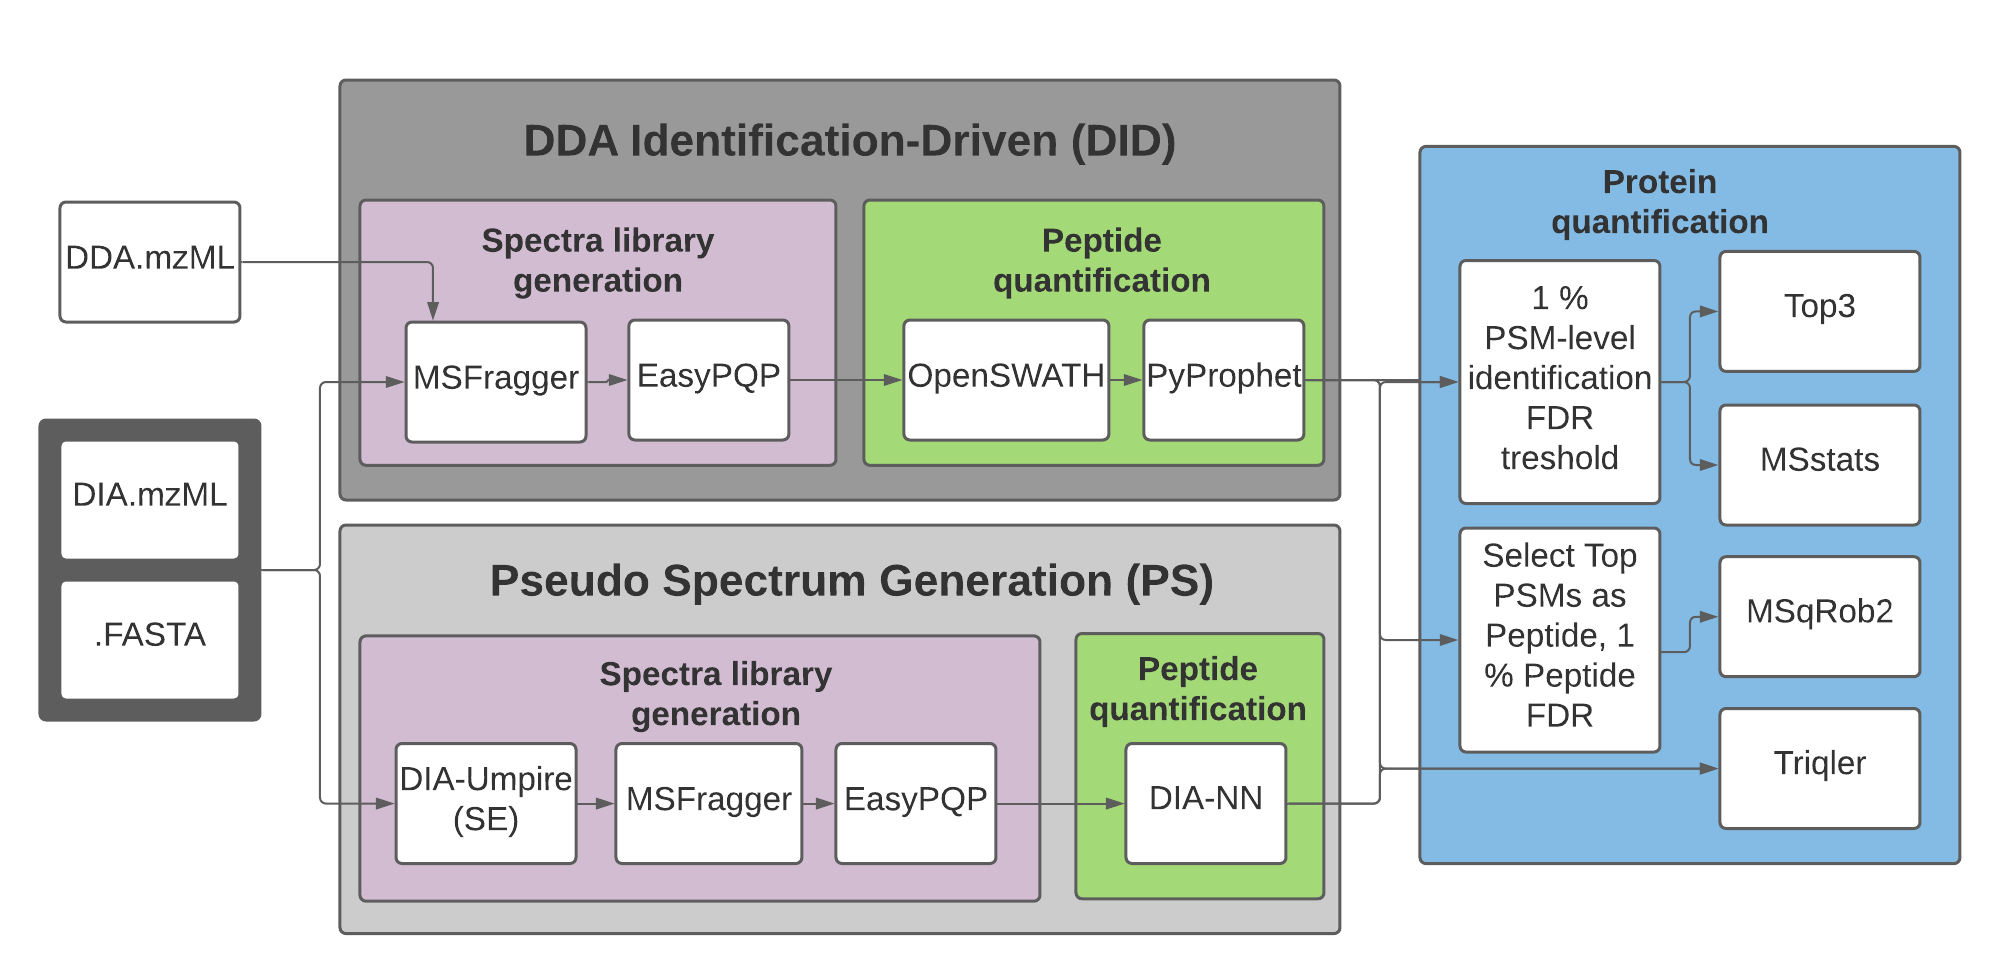
\includegraphics[width=1.0\linewidth]{../../result/report_plots/DIA_benchmark_truncated.png} 
    \end{tabular}
        \caption{{\bf The DDA identification-driven matching (DID) and pseudo spectrum workflow pipelines (PS).} In the pipelines DIA-Umpire(SE), MSFragger and EasyPQP is run from Fragpipe (\protect\url{https://fragpipe.nesvilab.org/}). A threshhold at 1\% PSM-level identification FDR was used for filtering before protein summarization. Triqler integrates the idenfication error probability of the peptides in its model and therefore should not use filtered data when performing protein summarization. Top3, MSqRobSum and MSstats uses the standard procedure of peptide filtering before protein summarization.}   
      \label{fig:flowchart}
\end{figure}



\subsubsection*{DDA identification-driven (DID) spectral library}

%\todo{We need a better name for this. Both your piplines use Spectral Libraries. Could you call this one ``Identification-driven''}


For the DID workflow we searched the LFQBench provided DDA runs with MSFragger\cite{kong2017msfragger} with default settings (Precursor mass tolerance of [-20, 20] ppms, fragment tolerance of 20 ppms, Calibration and Optimization: "Max calibration, parameter optimization", isotope error: 0/1, Data type: DDA, Load rules: stricttrypsin, Cut after: KR, Cleavages: ENZYMATIC, Missed cleavages: 2, Clip N-term M: True, Peptide length of [7, 50], Peptide mass range of [500, 5000], Split database: 1, and allowing for oxidation on methionine and protein N-terminus modifier as variable modifications), and constructed a spectral library with EasyPQP \cite{easypqp} to from the DDA-search results with default setting (RT Calibration: "Automatic selection of a run as reference RT", RT Lowess Fraction: 0.1, UniMod annotation tol(Da), Fragment annotation tol(ppm): 15, and the default PSM-level treshold of 0.01, peptide-level FDR of 0.01, and protein-level FDR of 0.01). Decoys for the spectral library was generated with OpenSwathDecoyGenerator with pseudo-reverse method. The spectral library was subsequently matched to the DIA data with the OpenSwath Workflow and  PyProphet\cite{teleman2015diana} was used for computing false discovery rate (m\_score) for the peptide quantification. This resulted in a set of detected peptides together with their assesed peptide identification accuracies and abundance estimates.

%Two approaches were used for spectra library generation: DDA acquisition-based spectral library generation and Prosit-based spectral library generation using only .fasta file \cite{searle2020generating}. 
%For Prosit-based spectral library generation, the FASTA file was converted to Prosit input format using encyclopeDIA converter. Prosit\_2020\_intensity\_cid model was used as an intensity prediction model and Prosit\_2019\_irt was used as iRT prediction model.  \todo{I am confused, are there three different workflows?[ANSWER: Not at this moment, buy my ambition is to at some point get the encyclopeDIA going, perhaps we can skip this?]}


\subsubsection*{Pseudo Spectra generation (PS) spectral library}

For the PS workflow we also used the fragpipe software, employing DIA-Umpire to extract pseudo-spectra from the DIA data. The DIA-Umpire parameters was set to default values (MS1 PPM: 10, MS2 PPM: 20, Max Missed Scans: 1, Mass Defect Filter: True, RP max: 25, RF max: 500, Corr Treshold: 0, Delta Apex: 0.2, RT Overlap 0.3, Mass Defect Offset 0.1, Isotope Pattern: 0.3, MS1 SN: 1.1, MS2 SN: 1.1, Adjust Fragment Intensity: True). The pseudo-spectra were subsequently searched using using MSFragger with default settings (Precursor mass tolerance of [-20, 20] ppms, fragment tolerance of 20 ppms, Calibration and Optimization: "Max calibration, parameter optimization", isotope error: 0/1, Data type: DDA, Load rules: stricttrypsin, Cut after: KR, Cleavages: ENZYMATIC, Missed cleavages: 2, Clip N-term M: True, Peptide length of [7, 50], Peptide mass range of [500, 5000], Split database: 1, and allowing for oxidation on methionine and protein N-terminus modifier as variable modifications). A spectral library was build from the resulting PSMs using easyPQP with default setting (RT Calibration: ``Automatic selection of a run as reference RT'', RT Lowess Fraction: 0.1, UniMod annotation tol(Da), Fragment annotation tol(ppm): 15, and the default PSM-level treshold of 0.01, peptide-level FDR of 0.01, and protein-level FDR of 0.01). DIA-NN was used for peptide quantifications with settings specified in \url{https://fragpipe.nesvilab.org/docs/tutorial_DIA.html#quantify-with-dia-nn} (Protein inference: ``Off'', Quantification strategy: ``Robust LC (High accuracy)'', Precursor FDR (\%): 1.0, Protease: ``Trypsin/P'', Missed cleavages: 1, Maximum number of cariable modifications: 0, N-term M excision: True, C carbamidomethylation: True, Peptide length: [7, 30], Precursor m/z range: [300, 1800], Fragment ion m/z range: [200, 1800], Mass accuracy: 0.0, MS1 accuracy: 0.0, Scan window: 0, Use isotopologues: True, Remove likely interferences: True, Neural network classifier: ``Single-pass mode'', Protein inference: Genes, Cross-run normalization: ``RT-dependent'', Library generation: ``Smart profiling''). Too compute false discover rates DIA-NN uses a built-in custom implementation of the mProphet algorithm to compute $q$~values \cite{reiter2011mprophet, demichev2020dia}.
 
%For the PS workflow we also used the fragpipe software, employing DIA-Umpire to extract pseudo-spectra from the DIA data. The pseudo-spectra were subsequently searched using using MSFragger with a precursor mass tolerance of -20, 20] ppms, fragment tolerance of 20 ppms, and allowing for [M,[\^{}] variable modifications (M - oxidation on methionine and \^{} is a terminus modifier for protein N-terminal). \todo{This is confusing. Spell out what it means. Do you look for N-term methionines, or is it something different?} A spectral library was build from the resulting PSMs at the default PSM-level treshold of 0.01 using easyPQP. DIA-NN was used for peptide quantifications, a method that uses a built-in custom implementation of the mProphet algorithm to compute $q$~values \cite{reiter2011mprophet, demichev2020dia}.
 
 %The DIA-NN uses a built-in mProphet algorithm with decoy precursors to compute the $q$~values. \cite{reiter2011mprophet} \cite{demichev2020dia}. 

% VARIABLE MODIFICATION 
% https://github-wiki-see.page/m/Nesvilab/MSFragger/wiki/Setting-the-Parameters 

%\subsection*{Database searching}
%For both workflow we matched spectra and pseudo-spectra with MSFragger with parameters: [check parameters], and used peptide-prophet for statistical validation was performed by peptide prophet and protein prophet.


\subsection*{Protein summarization}

The peptide quantities was summarized to proteins using the average of the three most intense peptides (We call it Top3), MSstats, MSqRobSum and Triqler for both the DID spectral library and the PS spectra library pipelines. 

\subsubsection*{Top3}

We implemented a short script that for each protein selected the average of the 3 most abundant PSMs for each protein and sample. In samples only having two PSMs available these were also included, still represented by their average, however, samples having zero or one PSM for the protein were excluded. PSMs were filtered at an 1\% FDR before performing the Top3 protein summarization. 

\todo{Here you clearly state that you use peptide-level FDR. Yet you say that you use PSM-level FDR elsewhere.}

% res = triq_run.groupby("proteins")["intensity"].apply(lambda x: x.nlargest(3).mean() if len(x.nlargest(3)) >= 2 else np.nan).reset_index()

%We implemented a short script that for each protein selected the three, on average, most abundant peptides across the conditions and summarized their protein quantities.

\subsubsection*{MsStats}

We installed MSstats version 3.18.5 using R/Bioconductor (available at \url{https://www.bioconductor.org/packages/release/bioc/html/MSstats.html}). MSstats use feature-level data, allowing for multiple PSM hits per peptide identification. We filtered so that every peptide so that every protein had at least 2 peptides and a maximum of 10 peptides, and we tresholded with a \texttt{m\_score} of lower than 0.01 with the \texttt{SWATH2stats} package in R in the SL pipeline. This was done using the settings \_on\_max\_peptides = 10, filter\_on\_min\_peptides = 2 and filter\_mscore\_condition = 0.01. For the PS pipeline we created a script for performing the same conversion and PSM filtering procedure. The PS pipeline data was filtered on the \texttt{Q.Value} columns from the DIA-NN output file instead of \texttt{m\_score}. MSstats was run using the MSstats command \texttt{dataProcess}. The significance testing between conditions was performed using the MSstats function \texttt{groupComparison}.  

%\todo{This cant be the prefered way to run msstats. Change so that you select peptides with a 1\% identification FDR.}

\subsubsection*{MSqRobSum}
% Details on how to run MsqRobSum
% https://rdrr.io/github/statOmics/MSqRobSum/f/vignettes/msqrobsum.Rmd

We installed MSqRobSum version 0.9 using R/Bioconductor (available at \url{https://github.com/statOmics/MSqRobSum}). MSqRobSum takes peptide input. The output from OpenSwath and DIA-NN is at PSM-level. We filtered the data on 1\% identification FDR and then filter the data to peptide-level by selecting the top PSM hit as our peptide. The highest scoring PSMs are selected as our peptides, i.e. highest \texttt{m\_score} for OpenSwath and highest \texttt{Q.Value} for DIA-NN. MsqRobSum was run using the MSqRobSum command \texttt{msqrobsum}, mode was set to \texttt{msqrob}, contrast was set to \texttt{condition} and \texttt{group\_vars} was set to the species human, yeast and \textit{E.Coli}. The \texttt{formulas} variables was set to \texttt{c(expression ~ (1|condition) + (1|sample) + (1|feature), expression ~ (1|condition))} and mode was set to \texttt{msqrob}. %This means that the two models $y_{st} = \beta_0 + \beta_{condition} + \beta_{sample} + \beta_{feature} + \epsilon$ and $y_{st} = \beta_0 + \beta_{condition} + \epsilon$ was specified for MSqRobSum analysis. 
MSqRobSum uses \texttt{lme4} to contruct a linear-mixed model with random effect, but without fixed effect. The models specified in by the variable formulas the constructs the models $y = Z_1 \mu + \epsilon$ and $y = Z_2 \mu + \epsilon$, where $Z_1$ contains the random effects condition, sample and feature (peptides for protein) and $Z_2$ contains only a random effect for condition. Some proteins have only intensities from one peptide. This can cause the first model $y = Z_1 \mu + \epsilon$ parameters to fail to converge. For these proteins we use the reduced model $y = Z_2 \mu + \epsilon$.

% information about symbolic formula for lmer4
% https://stats.oarc.ucla.edu/other/mult-pkg/introduction-to-linear-mixed-models/
% http://www.stat.rutgers.edu/home/yhung/Stat586/Mixed%20model/appendix-mixed-models.pdf
% https://arxiv.org/pdf/1911.08628.pdf


% for information about lmer4 syntax
% https://stats.stackexchange.com/questions/13166/rs-lmer-cheat-sheet

%\todo{LK: what is meant with a modell failing, in this case?}

%We downloded MSqRobSum version 0.9 from \url{FIXME}.

%clear
\subsubsection*{Triqler}

We downloaded Triqler from \url{https://github.com/statisticalbiotechnology/triqler}. We used Triqler v0.6.1 for the tests described in this paper. Triqler was run with \texttt{fold\_change\_eval} parameter between 0 and 2.00 with 0.04 increments. As Triqlers model accounts for the uncertainty in the data, it takes unfiltered PSMs as input. The \texttt{searchScore} column should reflect increasing certainty in PSMs. Therefore we apply negative log-transform to the \texttt{m\_score} and \texttt{Q.Value} to indicate \texttt{searchScore} 

\subsubsection*{Multiple Hypothesis Correction}
There was a slight difference in some of the benchmarking metrics, as the multiple test correction is performed with $q$~value for Triqler and Top3, while MsStats and MSqRobSum uses Benjamini-Hochberger \cite{benjamini1995controlling} corrections. The $q$~value approach aims to give a unbiased estimator of FDR, while the Benjamini-Hochberger approach estimates the upper bound of the FDR. As a consequens, the statistics from MsStats and MSqRobSum should be slightly more conservative \cite{korthauer2019practical}.

%For the OSW-pipeline the recommended pipeline consisting of running TRIC feature alignment was used before MSstats and msqrob conversion \todo{If I recall correctly non of the features was actually aligned, but I will rerun the computations to double check}. For all other data we did not use TRIC aligned peptide data. 


\section*{Results}



\subsection*{Validations of properties of DIA peptide abundance}

Triqler was designed for handling DDA data, and it was hence essential to validate that some of the assumptions Triqler makes about peptide abundance data, also are true for DIA datasets.
We hence downloaded the LFQBench dataset and processed it with two different pipelines, and investigated the properties of the reported pepide abundances. DIA data is known to encompass a larger dynamic range than DDA data \citation{bilbao2015processing}. This could affect one of Triqles assumptions, that the noise structure is mainly multiplicative, i.e. that the standard deviation within a sample group is proportional to its mean. When investigating all the peptide abundance measurements at a 1\% PSM identification FDR from the TripleTOF6600 section of the LFQBench dataset, we found a relatively linear relation between standard deviation and mean (Supplementary Figure \ref{fig:uniform_offset_in_standard_deviation_boxplot}A-D). Further, Triqler assumes that the missing peptide abundance values follow a censored normal distribution, which is also roughly fullfilled by DIA data (See Supplementary Figure \ref{fig:fraction_missing_values}).


\subsection*{Summarizing peptides to protein concentrations}

We wanted to compare the performance of Triqler to that of other protein summarization methods. An inherent problem when comparing different protein summarization softwares is that the performance is affected by which protein inference structure is used, in a data set dependent manner \cite{serang2012recognizing}. For example, when reporting number of differentially abundant proteins in data sets from mixtures from whole-cell extracts, a protein inference scheme that infer any protein contain a detected peptide will report more differentially abundant proteins than more restrictive scheme that just report a parsimonous set of proteins. For such data sets there is no mechanisms restrictive mechanism detecting situations where non-present proteoforms are reported as long as they are part of and reported with protein abundance rates compatible to the right proteome. To alleviate, or at least minimize, this problem from our comparison, we restricted the searched FASTA files by removing proteins with shared peptides. This operation stived to give a fairer comparison of protein summarization regardless of the protein inference method.

Given the peptide abundances derived from the DID and PS workflows, we could now compare the performance of Triqler to the one of MSstats, MSqRobSum and Top3. Here we selected to run Triqler with a lower bound estimate as described in The\&K\"{a}ll \cite{the2021triqler}, which ended up as 0.76 for the spectral library data, and 0.48 for the pseudo-spectra enabled data.

\subsubsection*{Distributions of the estimated fold changes}

To get an overview of the results of the methods we first made histograms of the reported protein level fold-changes as reported by the compared methods in Figure \ref{fig:fc_histogram}. For the these plots we removed all error assements on protein-level. We observe that Triqler and Top3 has less bias than MSstats and MSqRobSum, by seeing that the apex of the distributions are centered more closely to the true values.  %MSqRobSum report a very large number of proteins at a fold-change of zero. %These peaks all have a false discovery rate of 1.00, and would normally be filtered away by tresholding. 

\begin{figure}[hbt]
    \centering
    \begin{tabular}{cc}
	    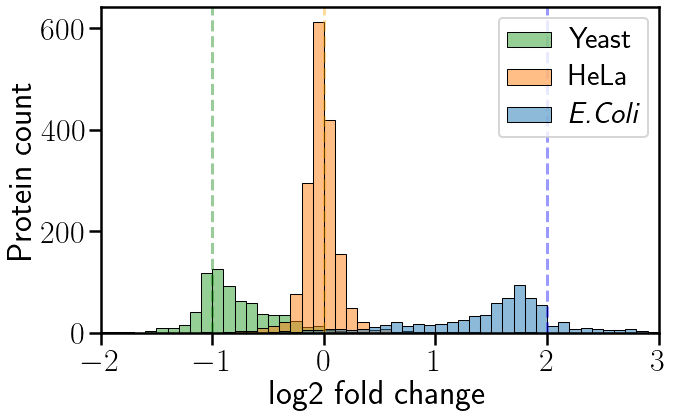
\includegraphics[width=0.4\linewidth]{../../result/report_plots_filtered/osw_triqler_intensity.png} & 
	    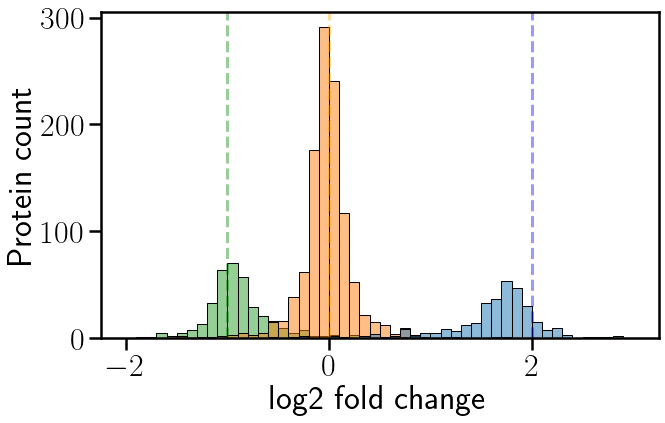
\includegraphics[width=0.4\linewidth]{../../result/report_plots_filtered/osw_top3_intensity.png} \\ 
        A & B \\ 
	    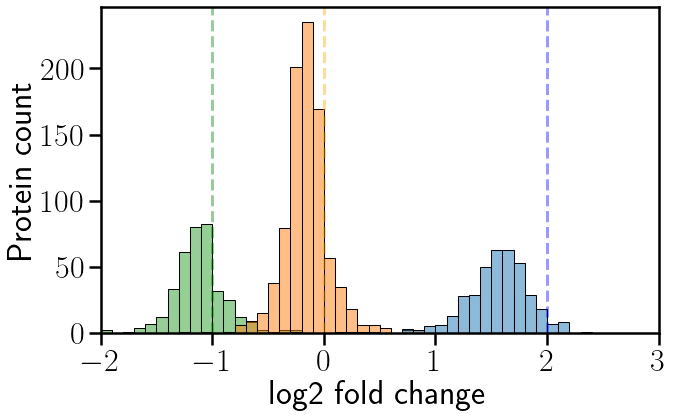
\includegraphics[width=0.4\linewidth]{../../result/report_plots_filtered/osw_msstats_intensity.png} & 
	    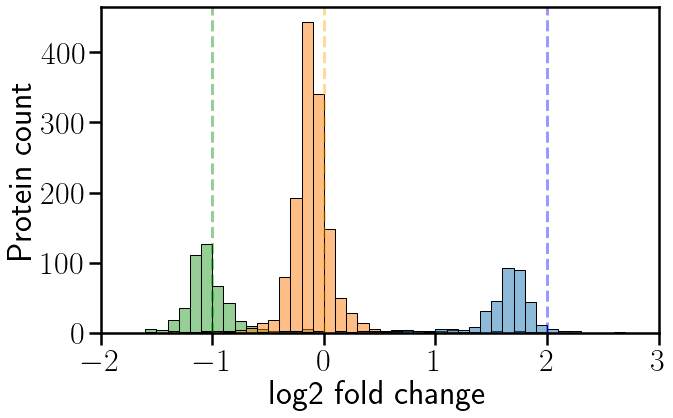
\includegraphics[width=0.4\linewidth]{../../result/report_plots_filtered/osw_msqrobsum_intensity.png} \\
        C & D 
    \end{tabular}
    \caption{{\bf Comparison of reported fold change distributions.} We used protein data from the DID spectral library pipeline and (A) Triqler, (B) Top3, (C) MSstats, and (D) MSqRobSum. The dashed lines indicates the true log2-fold change ratio between a specie and HeLa samples. We noted that the empirical densities of the protein counts are less biased for Triqler and Top3 than MSstats and MSqRobSum, the apex of their distribution were found closer to the true fold-change difference. \label{fig:fc_histogram}} %(D) MSqRobSum report a large fold change bin at 0. A majority of these valued have been filtered away using a tresholding procedure because the reported false discovery rate for the difference between groups was 1.0 for most values in this bin. \label{fig:fc_histogram}}
\end{figure}

\subsubsection*{Comparison of ability to discriminate differentially from equvalently abundant proteins}

The LFQBench set contain varying concentrations of {\em E. Coli} and Yeast concentrations in a background of HeLa-cells. As a first test of performance we hence compared the methods' ability to infer the differentially abundant {\em E. Coli} and Yeast protein as a function of the number of false positives from the HeLa-background, when varying the reported significance treshold from 0.0 to 0.1 with 0.001 increments (Figure \ref{fig:diff_vs_hela}). Overall, it seems like Triqler reports more differentially abundant protein for every non-differentially abundant protein for both the peptide abundances generated by the DID spectral library and PS spectral library pipelines. Surprisingly, Top3 performs has more true differentially abundant proteins for every false protein than MSstats. 


\begin{figure}[hbt]
    \centering
    \begin{tabular}{lclc} 
        A & 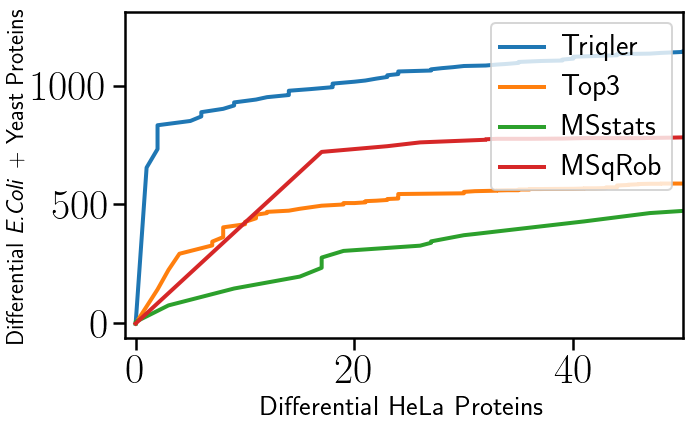
\includegraphics[width=0.45\linewidth]{../../result/report_plots_filtered/osw_de_human_vs_ecoli_and_yeast.png} & 
        B & 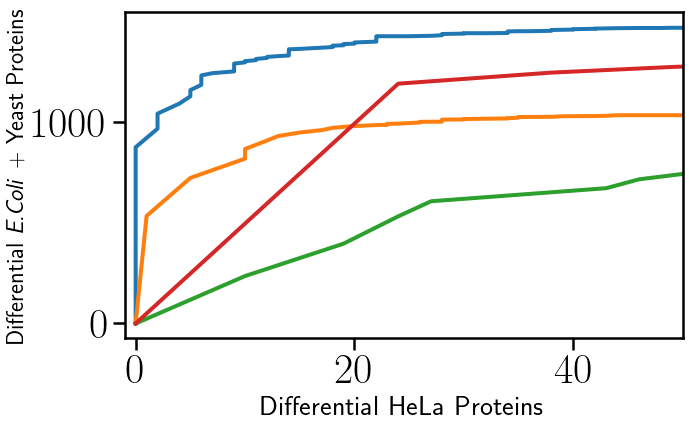
\includegraphics[width=0.45\linewidth]{../../result/report_plots_filtered/diann_de_human_vs_ecoli_and_yeast.png} \\ 

    \end{tabular} 
    \caption{{\bf Comparison of ability to differentiate proteins with differentiall abundance between conditions} We plotted the number of reported differentially abundant  {\em E. Coli} and Yeast proteins as a function of number of proteins from the HeLa background when sorting according to significance for (A) DDA generated spectral libraries and (B) DIA-Umpire geneated Pseudo spectra. For the test we selected a fold-change treshold of 0.64 for Triqler, because it is the rounded average of the lower bound for fold-change computed by Triqler (Supplement Figure \ref{fig:ability_to_differentiate_differentially_abundant_specie_vs_hela} shows differential abundance for each specie). \label{fig:diff_vs_hela}}
\end{figure}

\subsubsection*{Comparison of statistical calibration}

We subsequently set out to test the statistical calibration of the different summarization methods. We hence investigated the relation between the fraction of wrongly reported differential abundant proteins (i.e. the fraction of HeLa proteins among all reported differential abundant proteins), and each inference method's estimated false discovery rate (See Figure \ref{fig:frac_hela_vs_fdr}). We observe that Triqler, Top3 and MSqRobSum gives estimates that are close the true fold-change level than MSstats. This is somewhat surprising given that both MSstats and MSqRobSum are using the Benjamini-Hochberger corrections which are generally found more conservative that $q$~value estimates.

%We observed that Triqler and Top3 were reporting slightly more accurate estimates than MSstats and MSqRobSum. This is somewhat surprising given that both MSstats and MSqRobSum are using the Benjamini-Hochberger corrections which are generally found more conservative that $q$~value estimates.

\begin{figure}[hbt]
    \centering
    \begin{tabular}{cc} 
        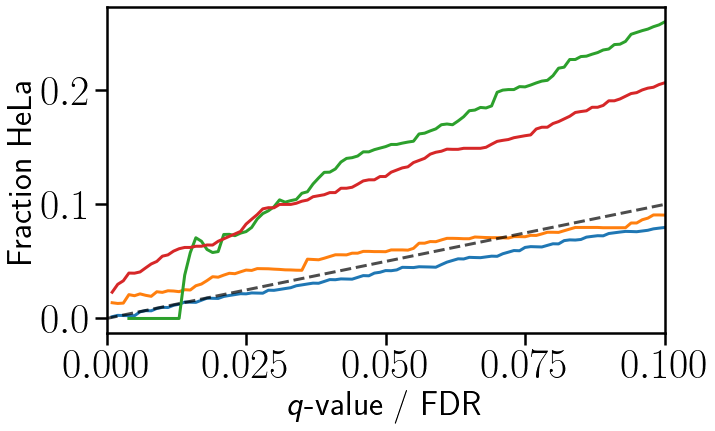
\includegraphics[width=0.5\linewidth]{../../result/report_plots_filtered/osw_FP_DE_all.png} & 
        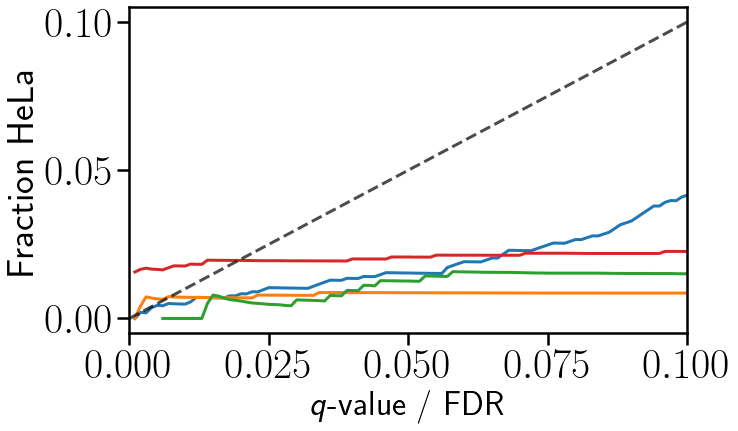
\includegraphics[width=0.5\linewidth]{../../result/report_plots_filtered/diann_FP_DE_all.png} \\
        A & B
    \end{tabular}
  \caption{{\bf Comparison of calibration of the compared summarization methods.} We plotted the fraction of reported differentially abundant HeLa proteins as a function of $q$~value treshhold for (A) DID spectral library pipeline and (B) PS spectral library pipeline. The multiple test correction is performed with $q$~value for Triqler and Top3, while Benjamini-Hochberger corrections was used for MSstats and MSqRobSum. \label{fig:frac_hela_vs_fdr}}
\end{figure}

\subsubsection*{Differential abundance reported by thr protein quantification tools.}

We also investigated the number of reported differential abundant proteins as reported by our four protein summarizatrion methods. The results can be found in Supplementary Figure \ref{fig:da_methods_esimate}. We note that a larger number of reported differentially abundant proteins were reported by e.g. MSqRobSum than Triqler, however, this was likely due to the more leanient FDR estmates by MSqRobSum.



\section*{Discussion}


Here we have shown that Triqler operates well for DIA data, despite originally intended for DDA data. We also find that Triqler outperforms other protein summarization methods on our engineered benchmark set, both in terms of sensitivity and accuracy in its error estimates. Triqler was also able to detect significantly higher number of differentially abundant proteins at a more accuratly reported false discovery rate, than the compared methods. 

The analytes in shotgun proteomics are peptides and not proteins or proteoforms. Nevertheless, most users of mass spectrometry use and will continue to find resons to report findings on a protein level. It makes sense to put efforts into better understanding of which protein inference tools to use at what occasion and how to summarize peptide abundances into protein relative concentration values.  Also, protein summarization gives lower variance than peptide-level analysis, and it reduces the amount of hypotheses tested and reduced the amount of missing values, which can have major impact on the quality of the analysis \cite{plubell2021can}.   

One important remark is that the sequence database that we used for matching the spectra was filtered so that only one protein per peptide was kept, to control for any difference in protein inference strategies used by our comparedprotein summarization methods. There is currently no consensus in how to handle multiple proteoforms in bottom-up proteomics. Hence, we believe that protein inference strategies that can account for multiple proteoforms would greatly benefit the field by improving the quality of the quantitative analysis. 

We do see some differences in how DIA and DDA peptide-level abundance data appear. For instance there are more missing values in DDA than DIA data. However, we find that qualitatively the types of data are similar, at least in the sense that Triqler's underlying assumption of missing values seem to be as valid for DDA and DIA data.

Lastly, we want to highlight the benefit and importance as datasets such as the one provided by Navarro et al. \cite{navarro2016multicenter}. These benchmarking datasets make it easy for the scientific community to investigate computational tools by providing a golden standard and significantly facilitates benchmark studies. 

\section*{Acknowledgements}


\section*{Funding}

This work was supported by grants from the Swedish Research Council (grant 2017-04030) 

\section*{Supporting information}

\bibliographystyle{plain}
%\bibliography{benchmark}
\bibliography{benchmark.bib}
\end{document}



